\chapter{Results of the 4.2 tonne-years exposure of the LUX-ZEPLIN experiment}\label{chap:WS2024Result}
In what follows, the latest WIMP search analysis from the LZ experiment is summarised. The analysis combines a 220 live-day exposure (WS2024) with the 60 live-day exposure from LZ's first WIMP search result (WS2022) \cite{LZ:2022lsv} to perform the most sensitive direct search for WIMPs to date \cite{LZCollaboration:2024lux}.

The WS2024 analysis is based on data collected between March 27, 2023 and April 1, 2024. Two distinct xenon flow configurations were used during this time, refereed to as the ``high-mixing'' and ``low-mixing'' states. The high-mixing state allows for homogeneous distributions of injected calibration sources. Whereas, the low-mixing state induces distinct regions of laminar flow throughout the detector where \textsuperscript{222}Rn-\textsuperscript{218}Po $\alpha$ decays are used to map the liquid xenon (LXe) velocity field. Of the WS2024 live time, 40.9 live-days are included when the detector was in a high-mixing state and the remaining 179.1 live-days, the detector was in a low-mixing state. The cathode, gate and anode electrodes establish the TPC drift field at 97~V/cm and extraction field at 3.4 kV/cm. The extraction field for the WS2024 science run was decreased with respect to the WS2022 science run configuration to reduce the dead time incurred from spurious electron and photon emission. The cathode voltage was lowered due to persistent light emission in the Skin region below the cathode.
The xenon gas maintained a stable (within 0.03\%) pressure of 1.860 bar(a) whilst the level of convective mixing of the LXe is controlled by regulating the temperature of the liquid entering the TPC from 177.9~K (high-mixing state) to 174.2~K (low-mixing state). The maximum drift time of the ionized electrons from interaction sites changes between mixing states from 1045~\textmu s (high-mixing state) to 1050~\textmu s (low-mixing state) and reduces the liquid height by $\sim0.2$~mm. Stable average electron lifetimes of 13.8~ms and 9.3~ms were maintain in low-mixing and high-mixing states respectively, far exceeding the maximum drift time in the TPC.

As mentioned in \autoref{sec:LZ/LZDAQ}, the data acquisition system uses trigger decision logic to primarily capture S2 pulses. The S2 trigger was optimized to increase sensitivity to low-energy events with an efficiency of 95~\% for S2 pulses corresponding to 3.5 extracted electrons.

Event waveforms are processed using LZap to find pulses and categorise interactions. Events are classified as single scatters (SS) if they have a single S1 preceding a single S2. High SS identification efficiency is crucial for the WIMP search since WIMPs will only scatter once when they pass through the TPC whereas background particles will likely multiple scatter. The SS identification efficiency is dependent on the S1 and S2 classification efficiencies. For a pulse to be classified as S1, a three-fold PMT coincidence requirement is used resulting in a SS S1 identification efficiency found to be $100\%$ for S1s $>35$~phd (8~keV). S1 and S2 signals express temporal and spatial variations due to changing detector conditions and are corrected for to produce standardised values, $\text{S1}c$ and $\text{S2}c$. The calibration sources outlined in \autoref{tab:LZ/CalibrationSources}, are used to determine the detector response model and pulse correction factors. S1 signals are normalised to the centre of the TPC volume and corrected by an $8\%$ average deviation from the absolute value. S2 signals are normalized to the radial centre of the liquid surface and additionally corrected for electron lifetime by correction average factors of $13\%$ and $7\%$, respectively.
Calibration sources (\textsuperscript{131m}Xe, \textsuperscript{83m}Kr and tritiated methane ($\text{CH}_3\text{T}$)) are used tune Noble Element Simulation Technique (NEST) \cite{NEST2011} model of the LZ detector to determine the detector response. The resulting photon gain $g_1$ is $0.112\pm0.002$~phd/photon and electron gain $g_2$ is $34\pm0.9$~phd/electron. NEST is also used to define ER and NR band medians and widths.

Candidate events for the WIMP search analysis are selected if they are classified as SS; located within the fiducial volume (FV); pass S1 and S2 pulse, live-time exclusion and veto coincidence selections and they lie within the WIMP region of interest (ROI). The WIMP ROI is defined such that $\text{S1}c$, $\text{S2}c$, and S2 pulse sizes are in a range of $3<\text{S1}c<80$~phd, $\text{S2}>645$~phd, and $\text{log}_\text{10}(\text{S2}c)<4.5$. 

External backgrounds are suppressed by the FV selection, illustrated in \autoref{fig:WS2024Result/fig1}. SS events which have a drift time, $t_\text{d}$, in the range between $1034\,(1030)<t_\text{d}<71$~\textmu s in the low(high)-mixing states are selected. Due to elevated radioactivity of the TPC field cage resistors, events which a have a reconstructed position $(x,y)$ within 6~cm of the troublesome resistors are excluded. The radial boundary of the FV follows a contour of the measured wall background event rate and is a function of both depth and azimuthal angle. The fiducial mass of the LXe is determined using the fraction tritium calibration events found in full active volume within the FV as $5.5\pm0.2$ tonnes.
\begin{figure}[t!]
    \centering
    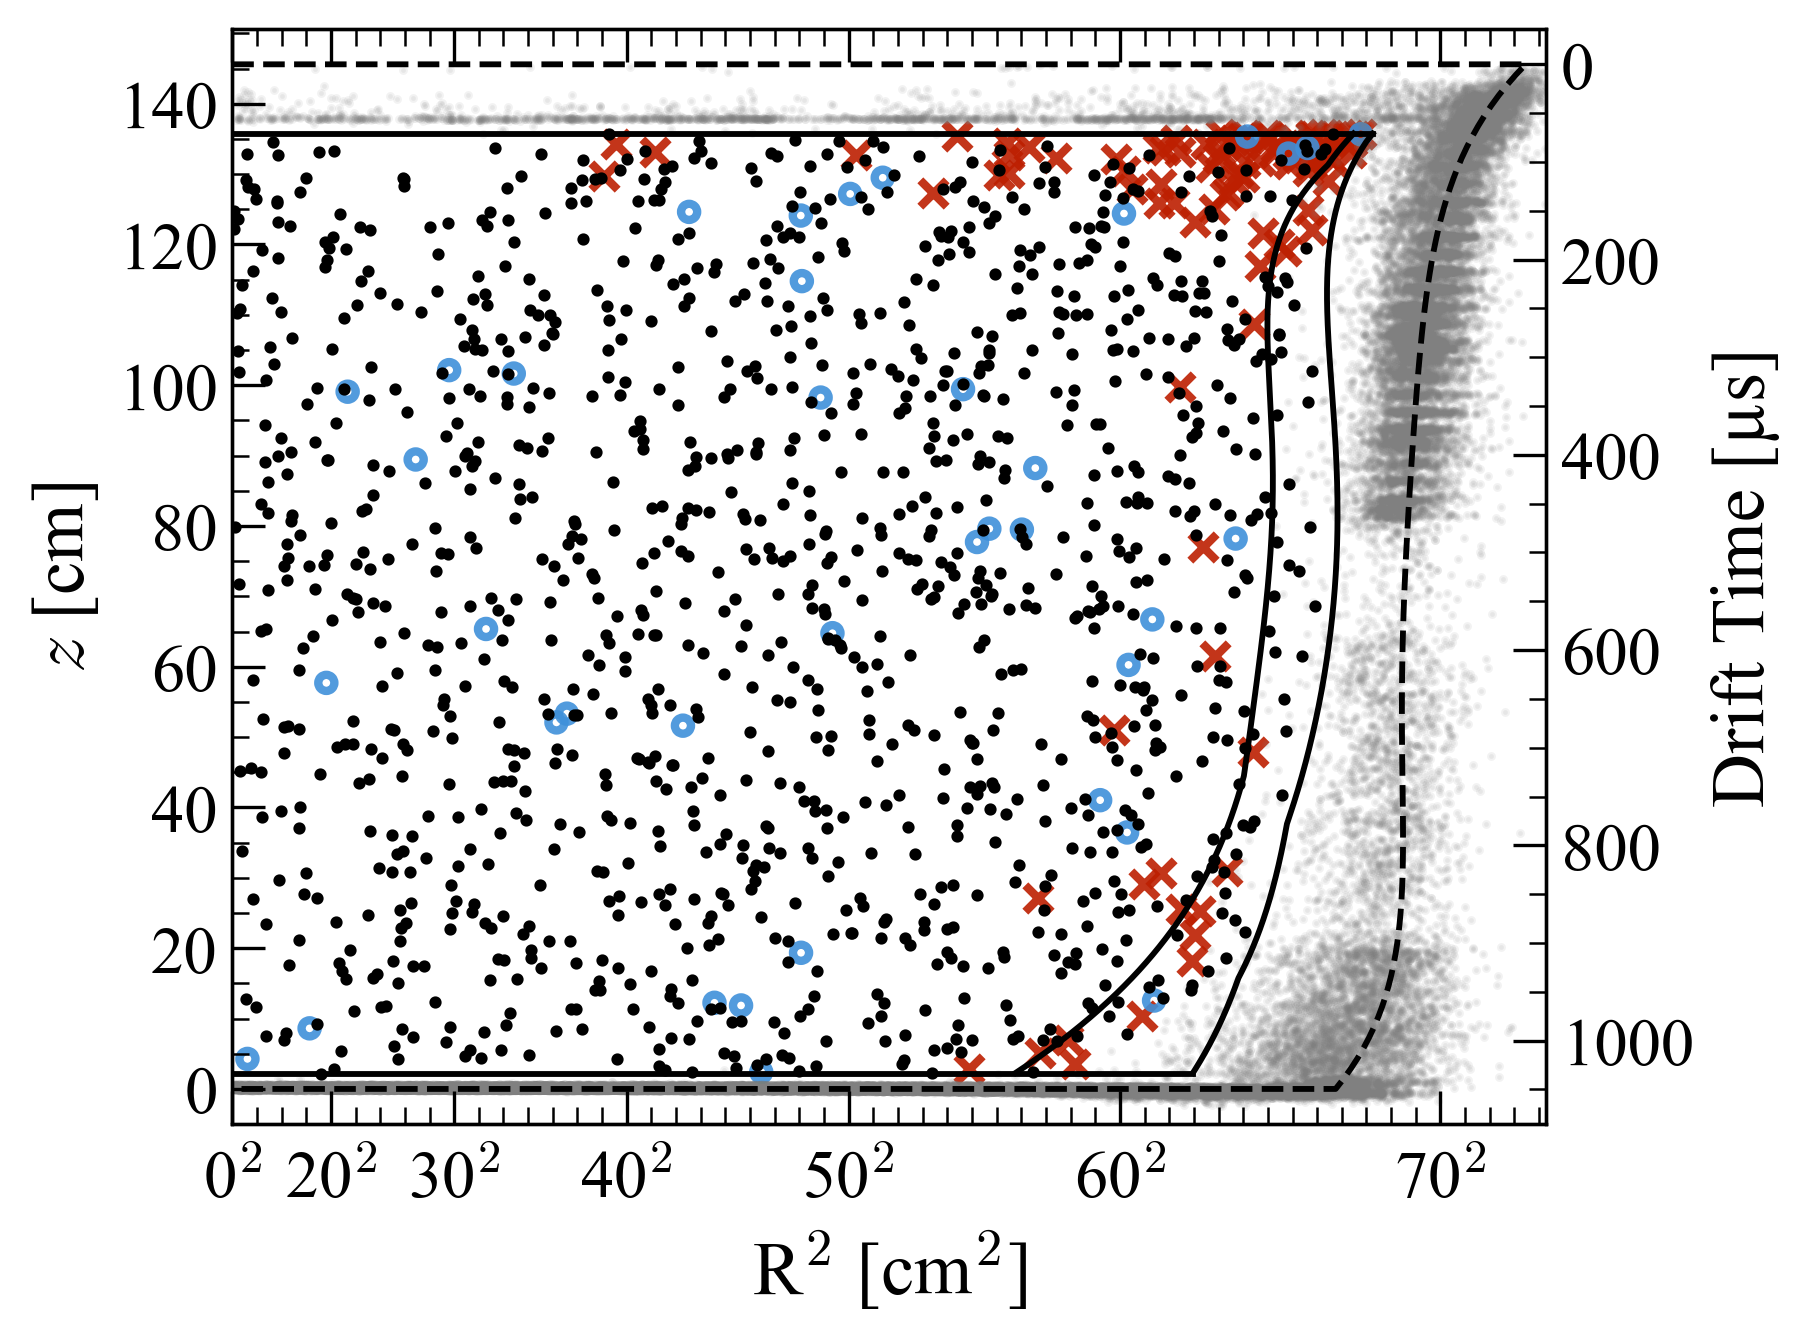
\includegraphics[width=0.7\linewidth]{figures/WS2024Result/figure1.png}
    \caption[Data from WS2024 reconstructed in $\text{R}^2$ and $z$ in the TPC.]{Data from WS2024 reconstructed in $\text{R}^2$ and $z$, in black with all analysis cuts applied, and in gray outside the FV without veto coincidence cuts. Red crosses and blue circles represent events that are vetoed by the prompt and delayed veto coincidence cuts, respectively. The dashed line shows the active volume, averaged over azimuth, and the two solid lines depict the FV, at the azimuths of its smallest and largest radial extent. Figured reprinted from Ref.~\cite{LZCollaboration:2024lux}.}
    \label{fig:WS2024Result/fig1}
\end{figure}
Accidental coincidence events are removed by cuts based on S1 and S2 pulse characteristics in-which random pairs of S1 and S2 pulses are classified as true SS interactions. Isolated S1 and S2 pulses are attributed to several sources, such as interactions in charge and light-insensitive regions of the TPC, spurious photon emissions, or delayed emission of electrons.

Live-time cuts excluded period with higher than average incidences of accidental coincidences due to elevated pulse rates \cite{LZCollaboration:2024lux}. Hold off times are imposed after large S2 pulses to remove events where delayed ionisation or correlated light emission is observed. One particular live-time cut which the author was responsible for developing for the WS2022 science run \cite{LZ:2022lsv} and subsequently optimised for the WS2024 science run was the ``muon hold off veto''. The study to develop this cut and the additional optimisation is described in \autoref{sec:Muons/MuonVeto}.

The veto coincidence cuts reject events which are accompanied by coincident signal in the Skin and/or OD. This selection represents the culmination of the efforts by the author to support the WIMP search analysis and the development of this selection is described in \autoref{chap:VetoEfficiency}. To refresh the readers knowledge of the veto coincidence selection, a description of the cuts follows. 
The veto coincidence selection is divided into two categories, prompt and delayed, for both the Skin and OD. Prompt cuts target $\gamma$-rays and fast neutrons, by removing events with pulses in the OD (Skin) of size $>4.5\,\text{phd}\,(>2.5\,\text{phd})$, PMT coincidence $>5\,(>2)$ within 0.3~\textmu s (0.25~\textmu s) of the S1. Delayed cuts target neutrons, which thermalize and capture on Gd or H in the OD with the release of an $\sim8~\text{MeV}$ $\gamma$-ray cascade. Events with pulses in the OD (Skin) of energy $>200~\text{keV}\,(>300~\text{keV})$ within 600~\textmu s after the S1 pulse are removed. The veto coincidence selection removes $3\%$ of collected livetime due to unrelated interactions in the veto detectors and the TPC. The veto efficiency for AmLi and DD calibration sources is measured to be $(89\pm3)\%$. Neutrons produced through spontaneous fission and ($\alpha$,n) reactions can be more effectively vetoed as they are typically higher in energy and are often accompanied by additional neutrons and $\gamma$-rays. The efficiency to veto background neutrons was determined through the comparison between simulations and calibration sources, indicating a neutron tagging efficiency of  $(92\pm4\%)$. The method to determine the associated uncertainty on the efficiency is described in \autoref{sec:VetoEff/BkgNeutronEff}.
The inclusion of the veto selection is apparent by the high density of veto tagged events shown in \autoref{fig:WS2024Result/fig1} and the ability for LZ to increase the FV of the TPC through wall background rejection using the veto detectors. This corresponds to a $40\%$ increase in exposure and is the most crucial impact of the authors efforts on the WS2024 science run. Without the veto selection cuts, the optimum method to remove the events highlighted in \autoref{fig:WS2024Result/fig1} would be to remove that portion of the target mass entirely, which would result in a reduced fiducial mass of 3.2~tonnes.

The cumulative effect of the event detection, data selection and reconstruction efficiencies on the NR signal is shown in \autoref{fig:WS2024Result/fig2}.
\begin{figure}[t!]
    \centering
    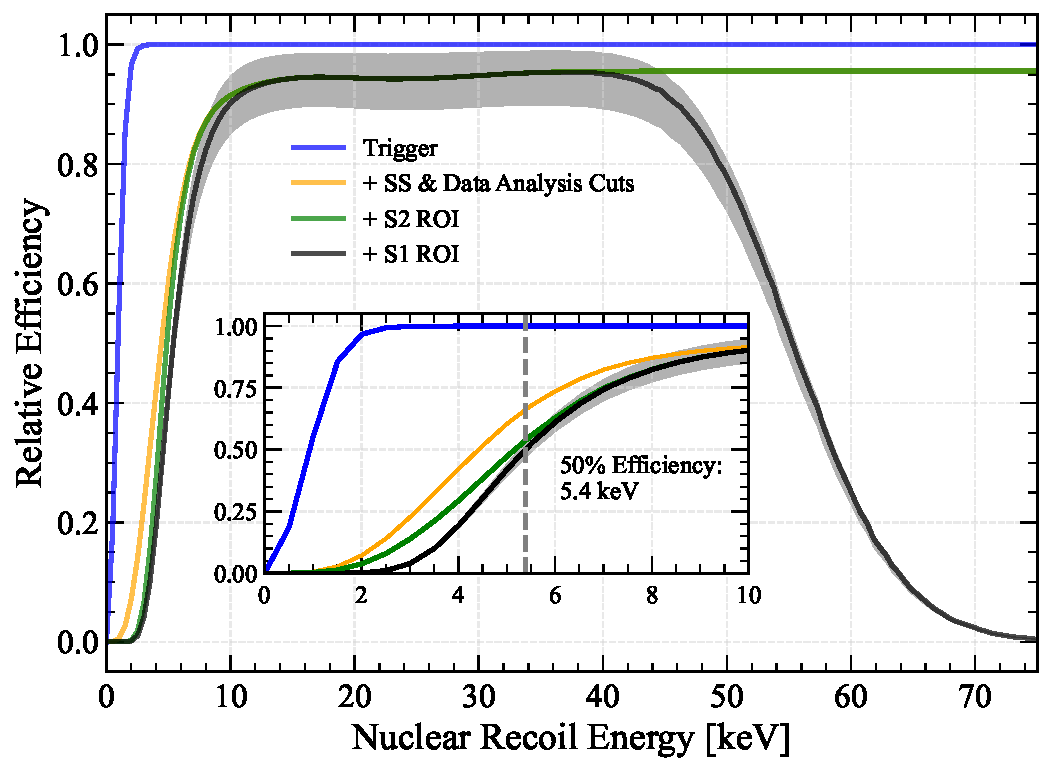
\includegraphics[width=0.7\linewidth]{figures/WS2024Result/figure2.pdf}
    \caption[Energy-dependent NR signal efficiency in the WS2024 analysis.]{Energy-dependent NR signal efficiency in WS2024 following the sequential application of the S2 trigger (blue); SS reconstruction and analysis cuts (orange); S2 ROI (green) followed by the S1 ROI (black). The insert shows the $50\%$ efficiency at 5.4~keV. The uncertainties are the combined statistical error of selections evaluated using different calibration data sets. Figured reprinted from Ref.~\cite{LZCollaboration:2024lux}}
    \label{fig:WS2024Result/fig2}
\end{figure}
A bias mitigation strategy is adopted for the WS2024 science run. Artificial, WIMP-like events are injected into the data at random times, this process is referred to as ``salting''. S1 and S2 pulses from tritium and AmLi calibration data sets are combined to generate salt events. An expected NR energy deposition is drawn from a parent distribution consisting of the sum of an exponential (WIMP-like) and a flat spectrum. Pairs S1 and S2 pulses which best match this energy deposition are chosen to be used as salt. The distribution of the salt events in the data set is kept hidden from the analysers for the entirety of the analysis and only revealed following the final definition of the data selection criteria and likelihood models. Eight salt events were injected and only one event was removed by the analysis cuts. This result is consistent with the NR signal efficiency. The salting model is described in detail in Ref.~\cite{LZCollaboration:2024lux}.

Following the application of all data selections and salt removal, 1220 events remain in the 3.3 tonne-year exposure of the WS2024 science run. These events are shown in \autoref{fig:WS2024Result/fig1} and \autoref{fig:WS2024Result/fig3}. A likelihood model is used to analyse these events using the $\{\text{S1}c,\text{log}_{10}(\text{S2}c)\}$ observables. NEST and event simulations \cite{LZ_SIMS} are used to generate signal and background models, whilst the accidental coincidence background model was generated using the same data-driven method used for the WS2022 result \cite{LZ:2022lsv}. The expected background counts are shown in \autoref{tab:WS2024Result/BackgroundCounts}.

The largest ER background contribution in the WS2024 exposure originates from $\beta$-emitting isotopes in the LXe bulk. The contribution of \textsuperscript{39}Ar and \textsuperscript{85}Kr to the ER background is estimated using \textit{in situ} xenon sampling measurements to indicate the concentration of \textsuperscript{nat.}Ar and \textsuperscript{nat.}Kr. Residual tritium and \textsuperscript{14}C activity following calibration injections is incorporated into the background model following the period of injection. Radon emanates from materials exposed to xenon and undergoes $\beta$-decay to \textsuperscript{214}Pb specifically from the \textsuperscript{222}Rn decay chain. This background is mitigated by the inline radon reduction system described in Ref.~\cite{marthurs:thesis}, however this is still the dominant ER background observed. A novel radon tagging method is used to identify events with a high likelihood of being a \textsuperscript{214}Pb decay. The method was developed using simulations of the movement of daughter atoms and ions built from observed flow vectors between \textsuperscript{222}Rn-\textsuperscript{218}Po $\alpha$-decay pairs. The radon tag can only be applied in the low-mixing state, where the flow can be modelled. Additionally, the radon tag can not be applied during periods after flow disturbances occur due to power outages and during gaps in data acquisitions. The remainder of the ER backgrounds are resultant of electron capture (EC) and double electron capture (DEC) decays in which energy is deposited via X-ray and Auger cascades. Preliminary measurements of the effects of these decays were performed with sideband datasets of Skin-tagged and multiple scatter (MS) decays of \textsuperscript{127}Xe and \textsuperscript{125}Xe which are produced \textit{in situ} via neutron activation following calibration campaigns.

The background model considers two sources to account for the background NR events: those arising those from neutrino interactions and from radioactive decays of detector components. The former are from CE$\nu$NS of solar and cosmic-ray generated atmospheric neutrinos. NRs that originate from ($\alpha$,n) and spontaneous fission (SF) reactions in detector materials can be vetoed by detecting scattering neutrons and/or associated $\gamma$-rays in the veto detectors. A side band data set of these vetoed events are used to derive an \textit{in situ} constraint of the number of neutron events. The selection for the veto side band was developed by the author and is described in \autoref{sec:VetoEff/efficiency}.
In the final statistical analysis, a side-band only fit returns an expectation of 0.0\textsuperscript{+0.2} SS counts. MS neutrons events tagged by the veto detectors in simulations of detector materials and data return expect neutron counts of $0.05\pm0.01$ and $0.3\pm0.2$ respectively.

\begin{table}[hbtp]
    \caption[The expected and best-fit counts for different sources in the 3.3~tonne-year exposure of WS2024]{The expected and best-fit counts for different sources in the 3.3~tonne-year exposure of WS2024, including a 40~GeV/$c^2$ WIMP signal. Table reproduced from Ref.~\cite{LZCollaboration:2024lux}.}
    \label{tab:WS2024Result/BackgroundCounts}
    \centering
    \begin{tabular}{lr@{}lr@{}l}
    \tabularnewline
    \hline
    \hline
    Source & \multicolumn{2}{l}{Pre-fit Expectation}
    & \multicolumn{2}{c}{Fit Result}\tabularnewline
    \hline \tabularnewline[-2.2ex]
    \textsuperscript{214}Pb $\beta$s &\centering 743 &~$\pm$ 88\phantom{0} &\centering  733 &~$\pm$ 34 \phantom{0}  
    \tabularnewline
    $^{85}$Kr + $^{39}$Ar $\beta$s + det. $\gamma$s &\centering 162  &~$\pm$ 22\phantom{0} &\centering 161 &~$\pm$ 21 \phantom{0} 
    \tabularnewline
    Solar $\nu$ ER& 102 &~$\pm$ 6 \phantom{0} & 102 &~$\pm$ 6 \phantom{0}
    \tabularnewline
    $^{212}$Pb + $^{218}$Po $\beta$s &\centering 62.7 &~$\pm$ 7.5 \phantom{0} &\centering 63.7 &~$\pm$ 7.4 \phantom{0} 
    \tabularnewline
    Tritium+ $^{14}$C $\beta$s &\centering 58.3  &~$\pm$ 3.3 \phantom{0} &\centering 59.7 &~$\pm$ 3.3 \phantom{0}
    \tabularnewline
    \textsuperscript{136}Xe $2\nu\beta\beta$ &	55.6 &~$\pm$ 8.3 \phantom{0} & 55.9 &~$\pm$ 8.2 \phantom{0} 
    \tabularnewline 
    \textsuperscript{124}Xe DEC & 19.4 &~$\pm$ 2.5  & 20.4 &~$\pm$ 2.4 
    \tabularnewline
    \textsuperscript{127}Xe +  \textsuperscript{125}Xe EC & 3.2 &~$\pm$ 0.6  & 2.7 &~$\pm$ 0.6 
    \tabularnewline
    Accidental coincidences	& 2.8 &~$\pm$ 0.6 & 2.6 &~$\pm$ 0.6 
     \tabularnewline
    $\textrm{Atm.}$ $\nu$ NR & 0.12 &~$\pm$ 0.02 & 0.12 &~$\pm$ 0.02
    \tabularnewline
    $^8$B$+hep$ $\nu$ NR & 0.06 &~$\pm$ 0.01 & 0.06 &~$\pm$ 0.01  
    \tabularnewline
   \hline \tabularnewline[-2.2ex]
    Detector neutrons &	\multicolumn{2}{l}{\phantom{00}$0.0^{+0.2}$} &  \multicolumn{2}{c}{$0.0^{+0.2}$} \tabularnewline[0.25ex]
    40~GeV/$c^2$ WIMP &\hfill &\phantom{0}--&  \multicolumn{2}{c}{$0.0^{+0.6}$} 
    \tabularnewline[0.25ex]
    \hline \tabularnewline[-2.2ex]
    Total & 1210 &~$\pm$ 91 & 1202 &~$\pm$ 41 \phantom{0} \tabularnewline
    \hline
    \hline
    \end{tabular}
\end{table}

The WS2024 exposure is divided into six mutually exclusive samples: high-mixing, where a radon tag is not possible; low-mixing, but with the radon tag inactive due to interruptions; low-mixing, active radon tag and radon-tagged, with a high probability to contain \textsuperscript{214}Pb decays; low-mixing, active radon tag and radon-untagged, with a lower probability to contain \textsuperscript{214}Pb decays; and events tagged by the Skin and OD delayed selection (discussed in detail in \autoref{sec:VetoEff4WIMPSearch}) \cite{LZCollaboration:2024lux}. The sixth sample represents the WS2022 dataset which contains the data and models from the 60 live-day WIMP search result \cite{LZ:2022lsv}. Nuisance parameters, which are allowed to float within their uncertainties, are the expected number of events for each background (listed in \autoref{tab:WS2024Result/BackgroundCounts}); neutron tagging efficiency; radon tagging efficiency; and the \textsuperscript{124}Xe charge to light yield ratio. The final set of events passing all selections cuts is shown in the upper left panel of \autoref{fig:WS2024Result/fig3_fig4}.

\begin{figure}[!ht]
	\centering
	\begin{subfigure}[b]{0.49\textwidth}
		\centering
		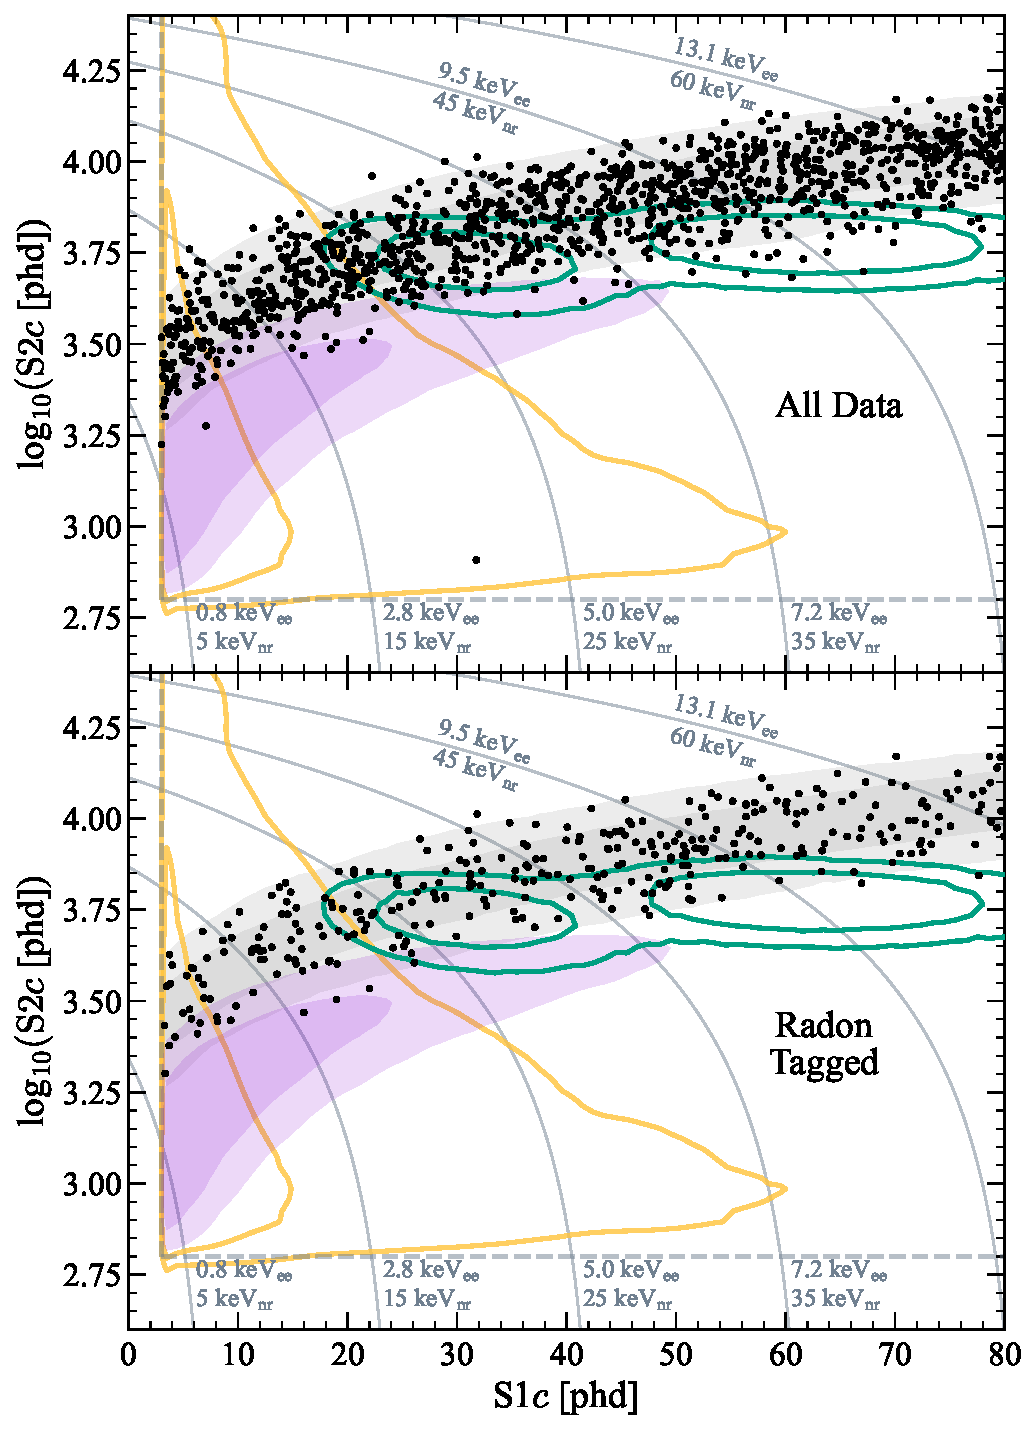
\includegraphics[width=\textwidth]{figures/WS2024Result/figure3.pdf}
        \caption{The final set of events passing all selection cuts with the panels distinguishing all events in WS2024 (top) from those that are radon tagged (bottom) are shown by the black points. Regions containing 68\% and 95\% of the ER portion of the background model and a 40~GeV/$c^2$ WIMP are shown with the dark and light gray and purple shading respectively. The best-fit \textsuperscript{124}Xe distribution and the accidental coincidence events are shown by the green and orange contours. Gray lines show contours of constant ER-equivalent ($\text{keV}_\text{ee}$) and NR-equivalent ($\text{keV}_\text{nr}$) energy \cite{LZCollaboration:2024lux}.}
		\label{fig:WS2024Result/fig3}
	\end{subfigure}
	\hfill
	\begin{subfigure}[b]{0.49\textwidth}
		\centering
		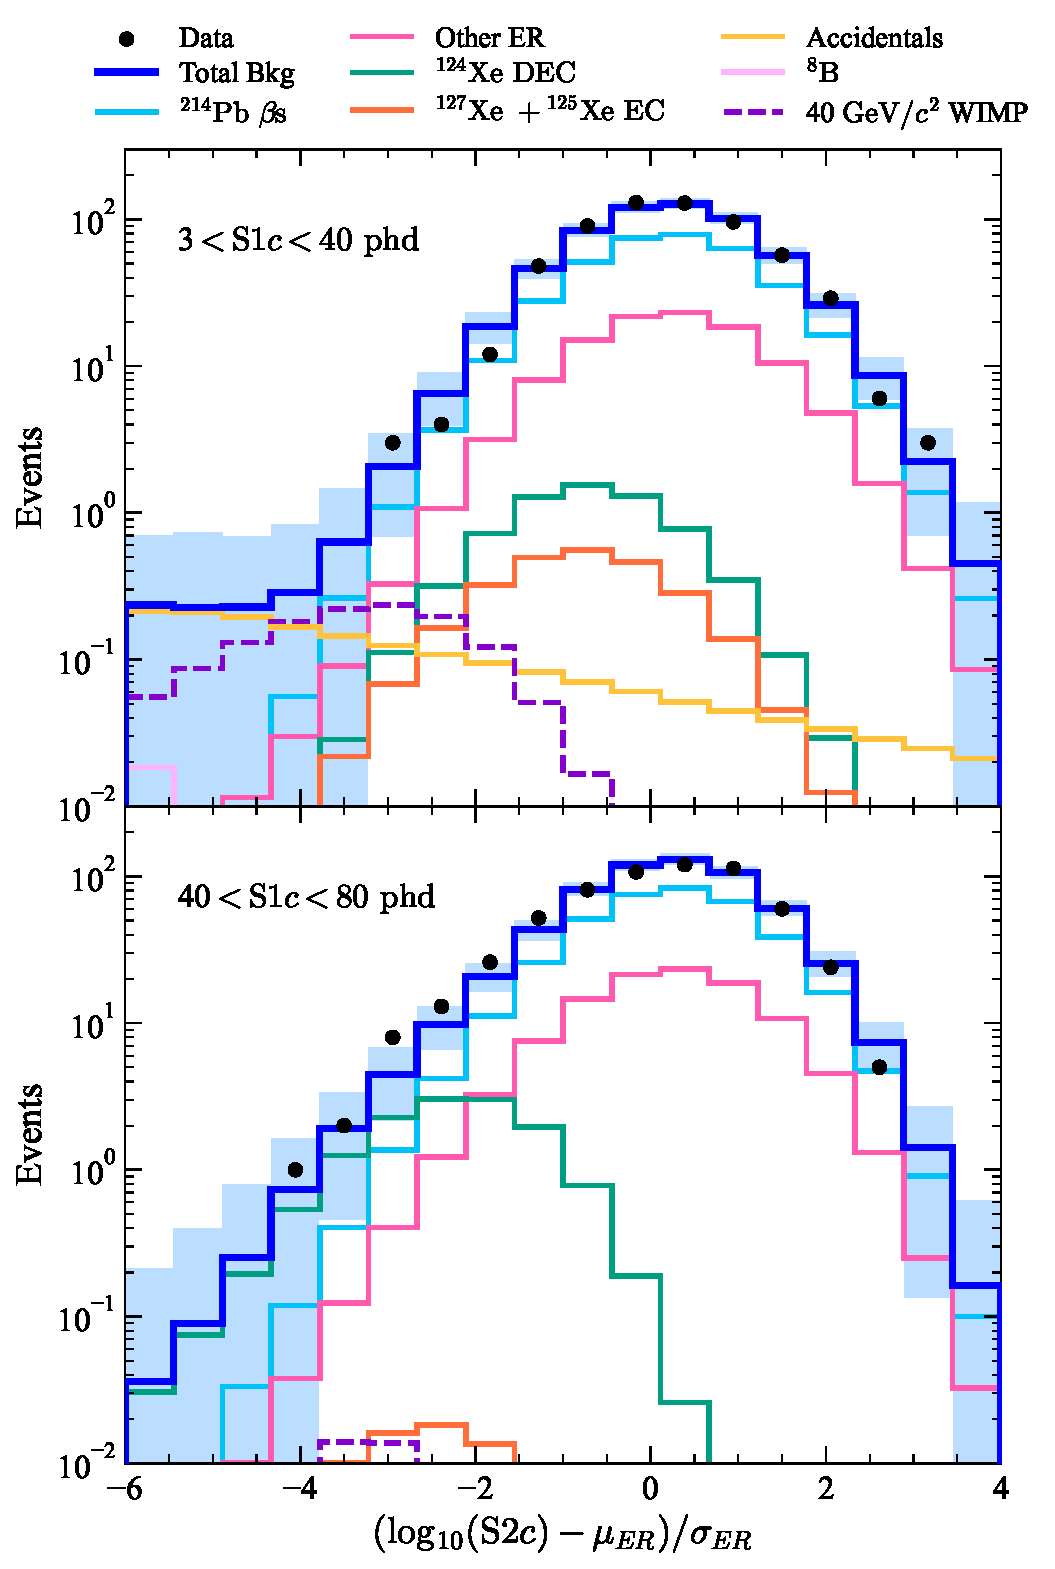
\includegraphics[width=\textwidth]{figures/WS2024Result/figure4.pdf}
		\caption{Comparison between data and the best-fit model for WS2024 corresponding to the values shown in \autoref{tab:WS2024Result/BackgroundCounts} for a background plus a 40~GeV/$c^2$ WIMP signal fit in a projection along the ER band median, normalized to the 1$\sigma$ band width. The upper and lower panels select the $\text{S1}c$ ranges 3–40 phd and 40–80 phd with p values of 0.55 and 0.59. The interval containing 68\% of the combined systematic and statistical uncertainties of the background model are depicted by the shaded band \cite{LZCollaboration:2024lux}.}
        \label{fig:WS2024Result/fig4}
	\end{subfigure}
	\caption[The final set of events passing all selection cuts with the panels distinguishing all events in WS2024 from those that are radon tagged. Alongside the comparison between data and best-fit model for WS2024 model is shown.]{\textbf{Left:} Events which pass all selection cuts (top) and those that are radon tagged (bottom). \textbf{Right:} Comparison between data and the best-fit model for WS2024 corresponding to the values shown in \autoref{tab:WS2024Result/BackgroundCounts} for a background plus a 40~GeV/$c^2$ WIMP signal fit in a projection along the ER band median, normalized to the 1$\sigma$ band width. Both figures are reprinted from Ref.~\cite{LZCollaboration:2024lux}.}
	\label{fig:WS2024Result/fig3_fig4}
\end{figure}

The best-fit number of WIMPs tested at all masses (between 9~GeV/$c^2$ and 100~TeV/$c^2$) for the combined WS2022+WS2024 analysis is zero. \autoref{fig:WS2024Result/fig4} shows the goodness of fit of the background-only model in a 1D projections along the ER band median. All samples show model-data agreement with a significance level of 0.05. The 90\% confidence level (C.L.) upper limit on the spin-independent WIMP-nucleon cross section as a function of mass is shown in \autoref{fig:WS2024Result/fig5}. The limit is power constrained at all WIMP mass to $1\sigma$ below the median expectation and the fluctuation along with the size of the constraint is largest between 20 and 50~GeV/$c^2$ \cite{LZCollaboration:2024lux}. This is due to the inclusion of the WS2022 data set from Ref.~\cite{LZ:2022lsv}, which exhibited an under-fluctuation of events in this region. The minimum of the limit curve is $2.2\times10^{-48}~\text{cm}^2$ at 40~GeV/$c^2$ while that of the median expected limit is $5.1\times10^{-48}~\text{cm}^2$ at 40~GeV/$c^2$ \cite{LZCollaboration:2024lux}.

\begin{figure}
    \centering
    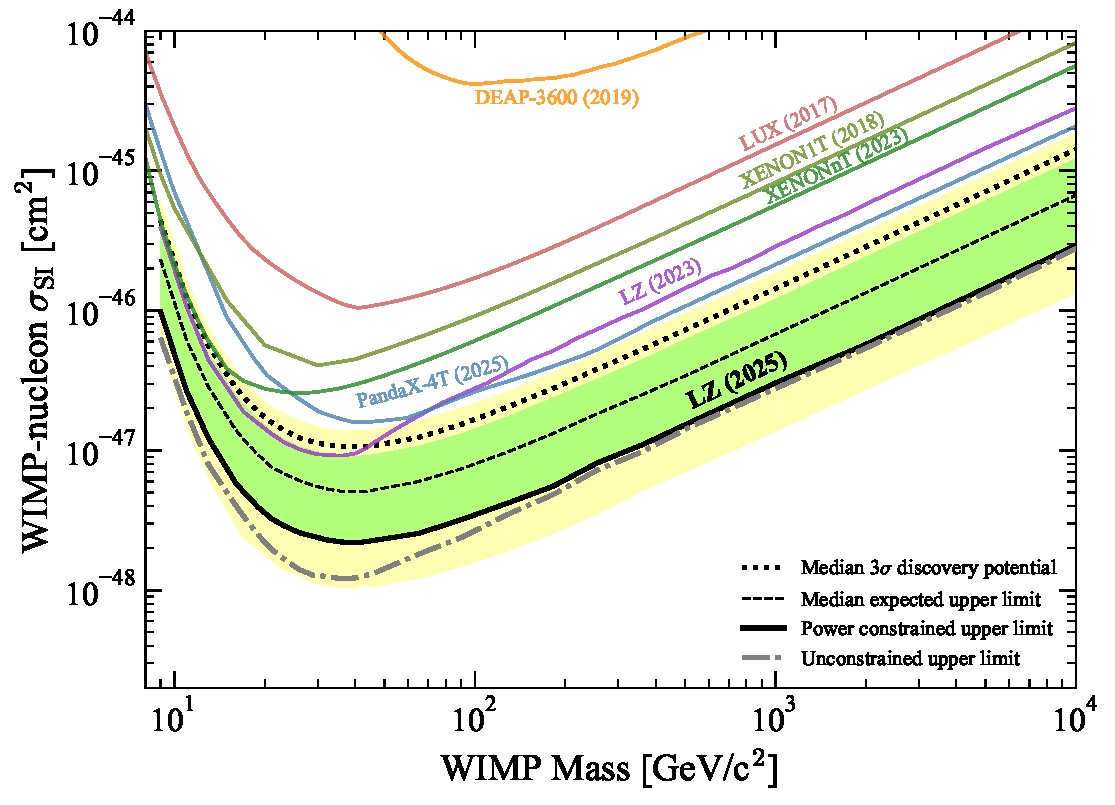
\includegraphics[width=0.7\linewidth]{figures/WS2024Result/figure5.pdf}
    \caption[Upper limits (90\% C.L.) on the spin-independent WIMP-nucleon cross section as a function of WIMP mass from the combined WS2024+WS2022 analysis (280 live days).]{Upper limits (90\% C.L.) on the spin-independent WIMP-nucleon cross section as a function of WIMP mass from the combined WS2024+WS2022 analysis (280 live days) are shown with a solid black line, with a $-1\sigma$ power constraint applied (LZ (2025)). The gray dot-dash line shows the limits without the power constraint; green and yellow regions show the range of expected upper limits from 68\% and 95\% of background-only experiments, while the dashed black line indicates the median expectation. The median $3\sigma$ observation potential from the post-fit model is shown as a dotted black line. Also shown are limits from WS2022 only \cite{LZ:2022lsv}, PandaX-4T \cite{PandaX-4T:2021bab}, LUX \cite{LUX:2016ggv}, all power constrained to $-1\sigma$; XENONnT \cite{XENONnTPres}, reinterpreted with a $-1\sigma$ power constraint; XENON1T \cite{XENON2018}, and DEAP-3600 \cite{DEAP:2019yzn}. Figure reprinted from Ref.~\cite{LZCollaboration:2024lux}.}
    \label{fig:WS2024Result/fig5}
\end{figure}

The LUX-ZEPLIN experiment has achieved world leading limits on SI WIMP-nucleon interactions by a factor of four for WIMP masses $>9$~GeV/$c^2$. The experiments continues to collect data towards a target 1000-day live time that will enable more sensitive searches for WIMP interactions whilst also probing new phenomena.